\chapter{Public Key Infrastructure (PKI)}\label{ch:publicKeyInfrastructure}

This chapter explains, how privacy in communication can be achieved and what infrastructure is needed to provide
encryption certificates for users.

\section{Public-Key Cryptography}\label{sec:publicKeyCryptography}
The goal of public key cryptography is to solve the \say{key-management problem with symmetric
cryptosystems}~\cite{diffie1976new}.
This problem with symmetric cryptography is the secure exchange of identical encryption keys, that can be easily
compromised in transport.
The mayor breakthrough of public-key and asymmetric cryptography was the usage of \say{two different keys - one public
and the other private}~\cite{schneier2007applied}, where the private key never needed to be transported.

In this cryptography, the public key is used for encryption and the private for decryption of messages.
Additionally, the private key can be used to sign messages, such that anyone with the public key can verify, that the
signature of this data was indeed issued by the corresponding private key.

Unfortunately, the public keys still need to be exchanges between users, which allows for so called man-in-the-middle
attacks, where an attacker exchanges Alice's public key with his own.
Bob now believes, he has Alice's public key, but actually, the middle man has broken the properties of public key
cryptography.

To solve the problem of such man-in-the-middle attacks, a system of trust was established.
In this system a trusted third party verifies, that the public keys are authentic.
This can in turn be verified with cryptographic signatures again to reduce the trust to as few manually exchanges keys
as possible.

\section{X.509 PKI}\label{sec:publicKeyInfrastructure}
The problem of which public keys to trust is nowadays handled with a so called Public Key Infrastructure (PKI).
This system consists of a combination of hard- and software, policies and procedures which organize the process of
certificate issuing, management and revocation.

The Internet Engineering Task Force (IETF) defines the PKI for X.509 in RFC5280~\cite{RFC5280}.
This formal model defines several key elements:
\begin{itemize}
    \item \textbf{End Entity} - Those are the actual users, i.e.\ people or devices, which can be identified with the
    subject field of a certificate.
    \item \textbf{Certificate Authority (CA)} - The entity which has the authority to issue certificates.
    A CA is an anchor of trust in the PKI and can sign certificates to bind public keys to End Entities.
    \item \textbf{Registration Authority (RA)} - An optional entity, to which CAs can transfer many administrative
    functions.
    \item \textbf{Certificate Revocation List (CRL)} - A list, which contains all revoked certificates, which should no
    longer be used, but which validity dates have not expired, yet.
    \item \textbf{Certificate Repository} - A database or directory service, which can be used to get certificates
    belonging to End Entities.
\end{itemize}

The process of acquiring certificates is a bit involved, but well defined:
The user first generates a key pair for asymmetric cryptography, with private and public key.
Then they send a Certificate Signing Request (CSR) to the CA\@.
This is basically a request to the CA so as to certify the digital identity or the user.
The CSR contains information about the applicant, like the distinguished name, their email addresses and their public
key which needs to be signed by the matching private key.

\begin{figure}
    \centering
    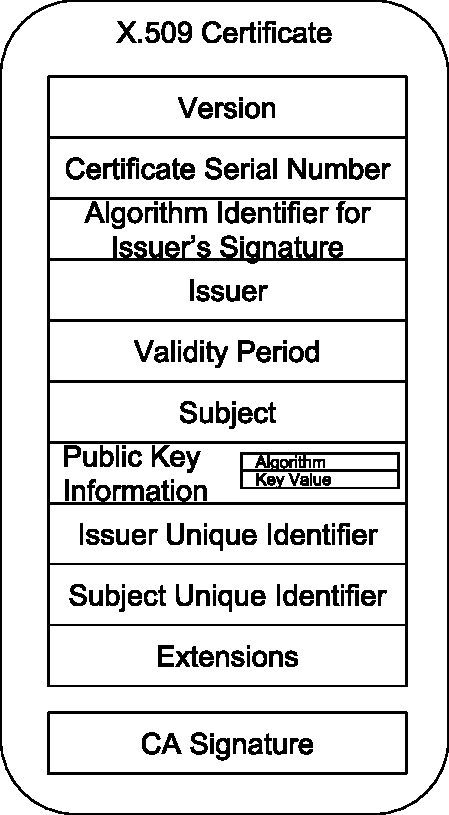
\includegraphics[width=0.3\textwidth]{figures/Structure_of_X509.pdf}
    \caption{Structure of a X.509 Certificate~\cite{jagdish2016certservice}}
    \label{fig:x509Structure}
\end{figure}

This CSR is then used to generate a valid X.509 public-key certificate.
The fields contained in those certificates are displayed in \Cref{fig:x509Structure}.

\section{Email Security}\label{sec:emailSecurity}

Emails, as defined in in RFC5322~\cite{RFC5322}, are unencrypted.
This is largely caused by the fact, that emails are somewhat a relic from ancient times of the internet, already
defined in 1977 as \say{ARPA NETWORK TEXT MESSAGES}~\cite{RFC0733}.
Since the message format has not changed dramatically since then, modern emails follow the same plain text structure.

Furthermore, the several associated protocols were inherently insecure, but have since received updates to use transport
encryption, like SMTP over TLS~\cite{RFC3207}.
Since this encryption is only a transport encryption, i.e.\ the message itself is transmitted encrypted over the wire,
but decrypted on each mail server, those attempts do not provide end-to-end security.
Truly confidential and authenticated messages are only possible using one of two competing end-to-end cryptographic
implementations, that operate on top of emails: PGP or S/MIME\@.

\subsection{PGP}\label{subsec:pgp}
Pretty Good Privacy (PGP) was first implemented by Philip Zimmermann in 1991~\cite{zimmermann1995official}.
PGP was one of the first readily available systems implementing public key cryptography.
PGP can be used for the most public key cryptography applications, like privacy, authentication, and digital signatures.

The modern variant of this software is open source and called OpenPGP\@.
It is the de-facto standard for PGP messages, but the message format was also formally specified in
RFC4880~\cite{RFC4880}.
Software support for PGP is usually good, e.g.\ in Mozilla Thunderbird via a plugin called \say{Enigmail}, but not
directly included.

\subsection{S/MIME}\label{subsec:s/mime}
S/MIME are the Secure/Multipurpose Internet Mail Extensions for signing MIME data and general encryption.
Initially, the format was defined by the RSA Data Security Inc.
But nowadays, the standard is also defined in an RFC, number 5750~\cite{RFC5750}.

In comparison to OpenPGP, most commonly used email clients, like Thunderbird, Microsoft's Outlook, and Apple Mail
support S/MIME without further plugins.
This makes S/MIME the most comfortable way to secure emails for users.
We will therefore focus on S/MIME in this work.

\section{Certificates at TUM}\label{sec:certificatesAtTum}
Certificate management in larger organizations is usually complex and confusing for the non technical user.
As an example, we can take a look at the existing certificate infrastructure at our own university: TUM\@.
There are several ways of acquiring certificates:

The \say{Leibniz-Rechenzentrum der Bayerischen Akademie der Wissenschaften} (LRZ in short) offers to sign
certificates~\cite{lrzpki}, which then can be used to secure servers hosted with the LRZ, but also for e-mail security.
The LRZ itself describes the situation as complicated, because of the \say{many other temporary installed solutions}
(\say{[da] sowohl am LRZ wie auch anderswo provisorische L\"osungen installiert worden sind}).

TUM IT-support also offers certification services~\cite{tumZertifikat}.
This system is the preferred way to acquire certificates for users, however the process is not adapted to the TUM
identity management, so the authentication of users needs to happen via physical verification of identity documents.

Additionally, TUMs Faculty of Informatics also runs a registration authority~\cite{inTumCertificates}.
This is certainly not a service intended for the general public, but only for members of the faculty.

All three of those certification solutions are based on the CA of the Deutsches For\-schungs\-netz (DFN)~\cite{dfnPki},
with each of the providers being a Registration Authority.
So, in theory any one certification method should have the same \say{trust}, however the certification requirements and
procedures significantly differ.
Furthermore, the process of generating public keys is not handled very well: LRZ provides a guide to generate keys with
the \lstinline{openssl} command line utilities, which disqualifies a lot of the users from using the RA\@.
The Faculty of Informatics generates the keys for their users - \emph{including private keys} - and stores them secured
with a RA generated passphrase.
This fails one of the basic requirements of public-key cryptography, that only the user should ever have access to the
private key.
TUM-IT uses the DFNs web interface to generate keys, which generates the keys in the users browser and encrypts them
with a user provided passphrase.
This process is a really good compromise between the ability of a layman to generate keys, while not breaking
cryptographic guidelines.
However, this web interface is not very accessible, especially on mobile devices, and additionally completely separated
from TUM infrastructure, such that basic integration within TUM workflows or many quality-of-life improvements can not
be made.
